\chapter{Background} \label{chap:background}

\section{Deep Learning} \label{sec:deeplearning}
\subsection{Motivations}
Deep learning has recently been highly successful in machine learning across a variety of application domains, including computer vision, natural language processing, and big data analysis, among others. For example, deep learning methods have consistently outperformed traditional methods for object recognition and detection in the IMAGENET Large Scale Visual Recognition Challenge (ISLVRC) since 2012 \cite{ILSVRC15}.
However, deep learning's high accuracy comes at the expense of high computational and memory requirements for both the training and inference phases of deep learning. Training a deep learning model is space and computationally expensive due to millions of parameters that need to be iteratively refined over multiple time epochs. Inference is computationally expensive due to the potentially high dimensionality of the input data (e.g., a high-resolution image) and millions of computations that need to be performed on the input data.

\subsection{Definitions}
As described in \cite{Goodfellow-et-al-2016}, the modern term "deep learning" goes beyond the neuroscientific perspective engineering applications on the current breed of machine learning models. It appeals to a more general principle of learning \textit{multiple levels of composition}, which can be applied in machine learning frameworks that are not necessarily neurally inspired. Deep learning is a subset of AI and machine learning and differs in that they can automatically learn representations from data such as images, video or text, to be used for classification without introducing hand-coded rules or human domain knowledge. Their highly flexible architectures can learn directly from raw data and can increase their predictive accuracy when provided with more data.
A deep learning prediction algorithm, consists of a number of layers, as shown in Fig. \ref{fig:dnn}.

\begin{figure}[tbp]
	\centering
	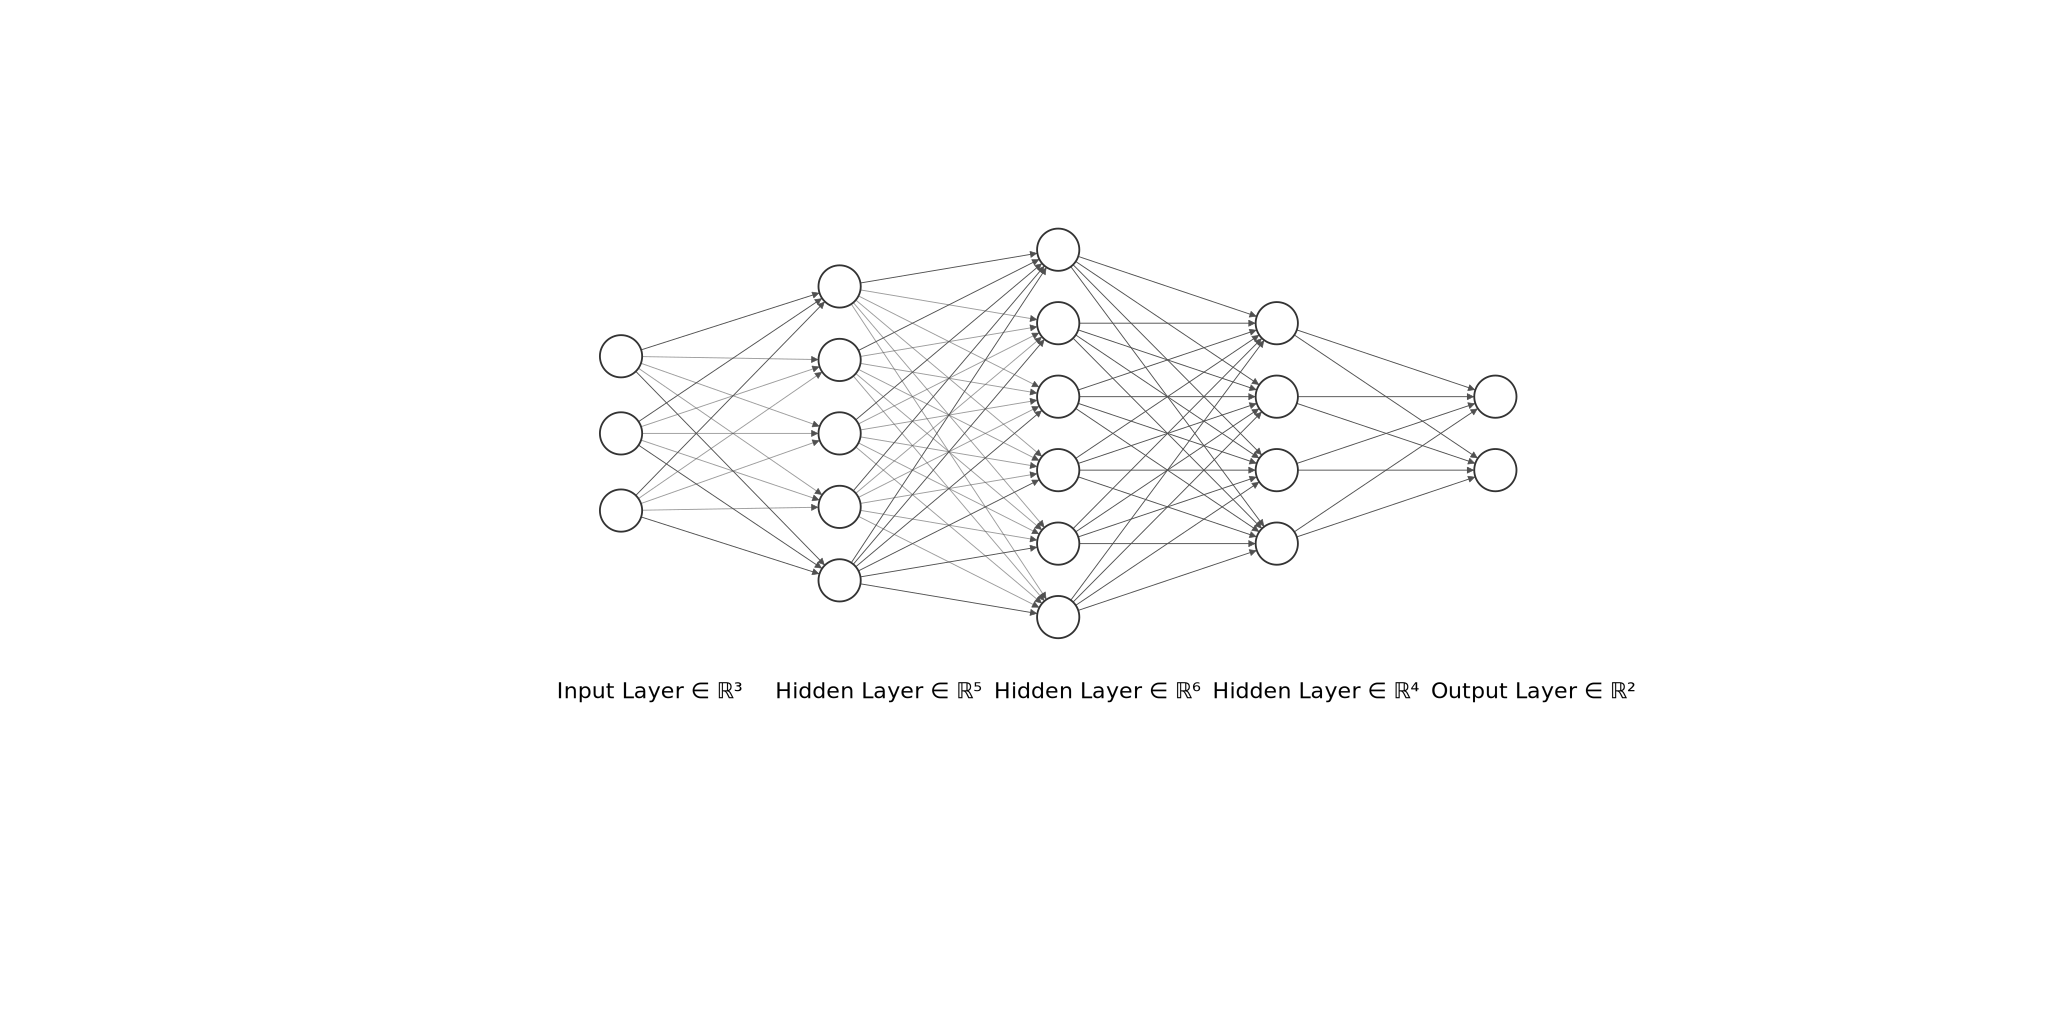
\includegraphics[width=0.9\linewidth]{images/nn}
	\caption[DNN example]{DNN example with image classification}
	\label{fig:dnn}
\end{figure}

In deep learning \textit{inference}, the input data pass through the node's layers in sequence, and each layer performs matrix multiplications on the data. The output of a layer is usually the input to the subsequent layer. After data are processed by the final (fully connected) layer, the output is either a feature or a classification value. When the model contains many layers in sequence, the neural network is known as a deep neural network (DNN). When the matrix multiplications include convolutional filter operations, the model is named convolutional neural networks (CNNs), which is common for image and video processing contexts. There are also DNNs designed especially for time series prediction; these are called recurrent neural networks (RNNs), which have loops in their layer connections to keep state and enable predictions on sequential inputs.

In deep learning \textit{training}, the computation proceeds in reverse order. Given the ground-truth training labels, multiple passes are made over the layers to optimize the parameters of each layer of matrix multiplications, starting from the final layer and ending with the first layer. The algorithm used is typically stochastic gradient descent (SGD).  In each pass, a randomly small subset of N input data ("mini-batch") from the training data set, is selected and used to update the gradients in the direction that minimizes the training loss (where the training loss is defined as the difference between the predictions and the ground truth). One pass through the entire training data set is called a training epoch \cite{ruder2016overview}.

There are some considerations to take into account: the first is that there are a large number of parameters in the matrix multiplications, resulting in many computations being performed and thus the latency issues that we see on end devices. The second is that there are many choices (hyper-parameters) on how to design the DNN models (e.g., the number of parameters per layer, and the number of layers), which makes the model design more of an art than a science. Different DNN design decisions result in tradeoffs between system metrics; for example, a DNN with higher accuracy likely requires more memory to store all the model parameters and will have higher latency because of all the matrix multiplications being performed. On the other hand, a DNN model with fewer parameters will likely execute more quickly and use less computational resources and energy, but it may not have sufficient accuracy to meet the application's requirements.


\subsection{Performance Measurement}
How can we evaluate the performance of a neural network?
Deep learning can be used to perform both supervised learning and unsupervised learning. The metrics of success depend on the particular application domain where deep learning is being applied. For example, in object detection, the accuracy may be measured by the mean average precision (mAP) \cite{ILSVRC15}, which measures how well the predicted object location overlaps with the ground-truth location, averaged across multiple categories of objects. In machine translation, the accuracy can be measured by the bilingual evaluation understudy score metric \cite{10.3115/1073083.1073135}, which compares a candidate translation with several ground-truth reference translations. 
Other general system performance metrics not specific to the application include throughput, latency, and energy. These metrics are summarized in Table \ref{tab:NN-Perfomance-Metrics}.
Designing a good DNN model or selecting the right DNN model for a given application is challenging due to the large number of hyper-parameter decisions.

\begin{table}[tbp]
	\centering
	\begin{tabular}{|l||c|} 
	\hline 
	 Metric & Unit	\\
	\hline
	Latency  &	s	\\
	Energy	& mW, J	\\
	Concurrent Requests Served	&	\#  \\
	Network Bandwidth	& Mbps			  \\
	Accuracy & Application Specific		\\
	\hline
	\end{tabular}
	\caption{Neural Network Performance Metrics\label{tab:NN-Perfomance-Metrics}}
\end{table}

Machine learning research typically focuses on accuracy metrics, and their system performance results are often reported from powerful server testbeds equipped with GPUs. For example, Huang et al. \cite{huang2016speedaccuracy} compared the speed and accuracy tradeoffs when running on a high-end gaming GPU (NVIDIA Titan X). The YOLO DNN model \cite{YOLO9000}, which is designed for real-time performance, provides timing measurements on the same server GPU.
Specifically targeting mobile devices, Lu et al. \cite{CNN-mobile} provided the measurements for a number of popular DNN models on mobile CPUs and GPUs (Nvidia TK1 and TX1). Ran et al.\cite{Ran-DNN-edge-video-analisys} further explored the accuracy-latency tradeoffs on mobile devices by measuring how reducing the dimensionality of the input size reduces the overall accuracy and latency. DNN models designed specifically for mobile devices, such as MobileNets \cite{howard2017mobilenets}, report system performance in terms of a number of multiply–add operations, which could be used to estimate latency characteristics and other metrics on different mobile hardware, based on the processing capabilities of the hardware.
Once the system performance is understood, the application developer can choose the right model. 


\subsection{Frameworks}
Several open-source software libraries are publicly available for deep learning inference and training on end devices and edge servers. Google's TensorFlow \cite{tensorflow2015-whitepaper}, released in 2015, is an interface for expressing machine learning algorithms and an implementation for executing such algorithms on heterogeneous distributed systems. Tensorflow's computation workflow is designed as a directed graph and utilizes a placement algorithm to distribute computation tasks based on the estimated or measured execution time and communication time \cite{abadi2016tensorflow}. The placement algorithm uses a greedy approach that places a computation task on the node that is expected to complete the computation the soonest. Tensorflow can run on edge devices, such as Raspberry Pi and smartphones. TensorFlow Lite was proposed in the late 2017 \cite{tensorflowlite}, which is an optimized version of Tensorflow for mobile and embedded devices, with mobile GPU support added in early 2019. 
Tensorflow Lite only provides on-device inference abilities, not training, and achieves low latency by compressing a pre-trained DNN model.
Caffe \cite{Caffe} is another deep learning framework, originally developed by Jia, with the current version, Caffe2, maintained by Facebook. It seeks to provide an easy and straightforward way for deep learning with a focus on mobile devices, including smartphones and Raspberry Pis. PyTorch \cite{NEURIPS2019_9015} is another deep learning platform developed by Facebook, with its main goal differing from Caffe2 in which it focuses on the integration of research prototypes to production development. Actually Facebook is working on the merge of Caffe2 and PyTorch frameworks.
GPUs are an important key element in efficient DNN inference and training. NVIDIA provides GPU software libraries to make use of NVIDIA GPUs, such as CUDA \cite{CUDA} for general GPU processing and cuDNN \cite{cuDNN} which is targeted toward deep learning. While such libraries are useful for training DNN models on a desktop server, cuDNN and CUDA are not widely available on current mobile devices such as smartphones. To utilize smartphone GPUs, Android developers can currently make use of Tensorflow Lite, which provides experimental GPU capabilities. To experiment with edge devices other than smartphones, researchers can turn to edge-specific development kits, such as the NVIDIA Jetson TX2 development kit for experimenting with edge computing, with NVIDIA-provided SDKs used to program the devices.



\subsection{Challenges}
Because of the required competences and effort to choose the best neural network and the best parameters that better fit the applications of our interest, there has also been much recent studies in automated machine learning, which uses artificial intelligence to choose which DNN model to run and tune the hyper-parameters. 
For example, Tan et al. \cite{tan2018mnasnet} and Taylor et al. \cite{taylor2018adaptive} proposed using reinforcement learning and traditional machine learning, respectively, to choose the right hyper-parameters for mobile devices, which is useful in edge scenarios.
As described in \cite{deepedgerev} many challenges remain in deploying deep learning on the edge, not only on end devices but also on the edge servers and on a combination of end devices, edge servers, and the cloud. For example parameters like latency, energy consumption and migration still the main challenges in the field of deep learning applied to the edge computing.



%%%%%%%%%%%%%%%%%%%%%%%%%%%%%%%%%%%%
\section{Edge Computing}
Today, an IoT solution has to cover a much broader scope of requirements. We see that in most cases, organizations opt for a combination of cloud and edge computing for complex IoT solutions. Cloud computing typically comes into play when organizations require storage and computing power to execute certain applications and processes, and to visualize telemetry data from anywhere. Edge computing, on the other hand, is the right choice in cases with low latency, local autonomous actions, reduced back-end traffic, and when confidential data is involved.

\subsection{Motivations}
As written in \cite{edgecomputingvision} there are at least three reasons to consider the adoption of edge computing. The first is that putting all the computing tasks on the cloud has been proved to be an efficient way for data processing since the computing power on the cloud outclasses the capability of the things at the edge. However, compared to the fast developing data processing speed, the bandwidth of the network has come to a standstill. With the growing quantity of data generated at the edge, speed of data transportation is becoming the bottleneck for the cloud-based computing paradigm.
The second reason is that almost all kinds of electrical devices will become part of IoT, and they will play the role of data producers as well as consumers, such as air quality sensors, LED bars, street lights and even an Internet-connected microwave oven. It is safe to infer that the number of things at the edge of the network will develop to more than billions in a few
years. Thus, raw data produced by them will be enormous, making conventional cloud computing not efficient enough to handle all these data. This means most of the data produced by IoT will never be transmitted to the cloud, instead it will be consumed at the edge of the network. Fig. \ref{fig:cloudarch} shows the conventional cloud computing structure.

\begin{figure}[tbp]
	\centering
	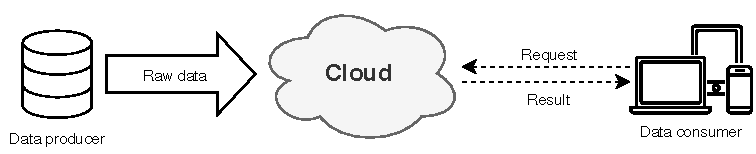
\includegraphics[width=0.9\linewidth]{images/cloudarch}
	\caption{Cloud computing paradigm}
	\label{fig:cloudarch}
\end{figure}

However, this structure is not sufficient for IoT. First, data quantity at the edge is too large, which will lead to huge unnecessary bandwidth and computing resource usage. Second, the privacy protection requirement will pose an obstacle for cloud computing in IoT. Lastly, most of the end nodes in IoT are energy constrained things, and the wireless communication module is usually very energy hungry, so offloading some computing tasks to the edge could be more energy efficient.
Another valid consideration to take into account is that in the cloud computing paradigm, the end devices at the edge usually play as data consumer, for example, watching a YouTube video on
your smart phone. However, people are also producing data nowadays from their mobile devices. The change from data consumer to data producer/consumer requires more function placement at the edge.


\subsection{Definitions}
Edge computing refers to the enabling technologies allowing computation to be performed at the edge of the network, on downstream data on behalf of cloud services and upstream data on behalf of IoT services. The rationale of edge computing is that computing should happen at the proximity of data sources. From a certain point of view, edge computing could interchangeable with fog computing \cite{openfog}, but edge computing focus more toward the things side, while the first focus more on the infrastructure side. Fig. \ref{fig:edgearch} illustrates the two-way computing streams in edge computing. In the edge computing paradigm, the things not only are data consumers, but also play as data producers. At the edge, the things can not only request service and content from the cloud but also perform the computing tasks from the cloud. Edge can perform computing offloading, data storage, caching and processing, as well as distribute request and delivery service from cloud to user. With those jobs in the network, the edge itself needs to be well designed to meet the requirement efficiently in service such as reliability, security, and privacy protection.

\begin{figure}[tbp]
	\centering
	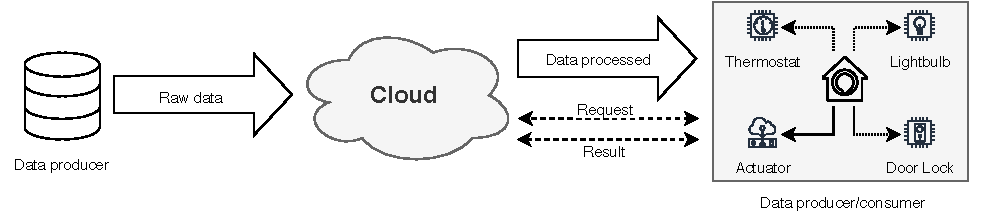
\includegraphics[width=0.9\linewidth]{images/edgearch}
	\caption{Edge computing paradigm}
	\label{fig:edgearch}
\end{figure}


\subsection{Performance Metrics}
In edge computing, we have multiple layers with different computation capability. Workload allocation becomes a big
issue. We need to decide which layer to handle the workload or how many tasks to assign at each part. There are multiple allocation strategies to complete a workload, for instances,
evenly distribute the workload on each layer or complete as much as possible on each layer To choose an optimal allocation strategy, there several optimization parameter to consider. These metrics are very similar to those described in \ref{sec:deeplearning}, including latency, bandwidth and energy. How to measure these performance is strongly dependent by the environment, resources and application case.


\subsection{Challenges}
In cloud computing, users program their code and deploy them on the cloud. Usually, the program is written in one programming language and compiled for a certain target platform, since the program only runs in the cloud. However, in the edge computing, computation is offloaded from the cloud, and the edge nodes are most likely heterogeneous platforms. In this case, the runtime of these nodes differ from each other, and the programmer faces huge difficulties to write an application that may be deployed in the edge computing paradigm.
Another important challenge is related to the \textit{naming}. In edge computing, one important assumption is that the number of things is tremendously large. At the top of the edge nodes, there are a lot of applications running, and each application has its own structure about how the service is provided. Similar to all computer systems, the naming scheme in edge computing is very important for development, addressing, things identification, and data communication. However, an efficient naming mechanism for the edge computing paradigm has not been built and standardized yet. Edge practitioners usually needs to learn various communication and network protocols in order to communicate with the heterogeneous things in their system.
In terms of \textit{service management} at the edge of the network, there are four fundamental features that should be supported to guarantee a reliable system, including differentiation, extensibility, isolation, and reliability.  
To protect the data \textit{security} and usage \textit{privacy} at the edge of the network, several challenges remain open. First is the awareness of privacy and security to the community: ip camera, health monitor, or even some Wi-Fi enabled toys could easily be connected by others if not protected properly. Second is the ownership of the data collected from things at edge. Just as what happened with mobile applications, the data of end user collected by things will be stored and analyzed at the service provider side. Third is the missing of efficient tools to protect data privacy and security at the edge of the network. The highly dynamic environment at the edge of the network also makes the network become vulnerable or unprotected and more tools are still missing to handle diverse data attributes for edge computing.


%%%%%%%%%%%%%%%%%%%%%%%%%%%%%%%%%%%%
\section{Robotics Tools and Platforms} \label{sec:Robotics-Tools-and-Platforms}
This section present the main robotics platforms analysed and explored during the development of this thesis.

\subsection{ROS}
The Robot Operating System (ROS) \cite{ROS}, is a open-source framework based on the component-based software engineering paradigm that provides the middleware for inter-process communication. Initially developed by the Stanford  Artificial Intelligence Laboratory its development continued at Willow Garage, a robotics research institute, and now it's maintained and improved under the action of the ORSF foundation \cite{ROS}. As a meta-operating system, ROS offers features such as hardware abstraction, low-level device control, implementation of commonly used functionalities, message communication between processes and package management. It uses an asynchronous publish/subscribing mechanism made possible by message standardisation and encapsulation that make the external interface of every node as general as possible, allowing quick nodes exchange and, thus, great architectural flexibility. Each independent block, called \textit{node}, executes a particular task of a process and can communicates with other nodes through \textit{topics}. This allows to create complex architectures by aggregating many simpler entities and simplifies the use of different tasks  or different methods for the same task. Additionally to the message-passing system, the core ROS component, called \textit{roscore}, maintains a global execution time for the nodes to achieve synchronisation. Each node executes separately with its own internal clock driven by the set execution rate. At every message sent/received, containing the internal time information, the core component updates the global time by following the execution status provided by these messages.
For more clarity about how ROS communication works an example is provided in figure \ref{fig:ros-nodes-topics}. When a publishing node will announce to the master that it is publishing over a topic and the subscribing node will say to the master that it want to listen to a topic. Then if the publisher
and the subscriber are on the same topic, the master will transfer data in order for the two other node to communicate directly via TCP/IP or UDP.

\begin{figure}[tbp]
	\centering
	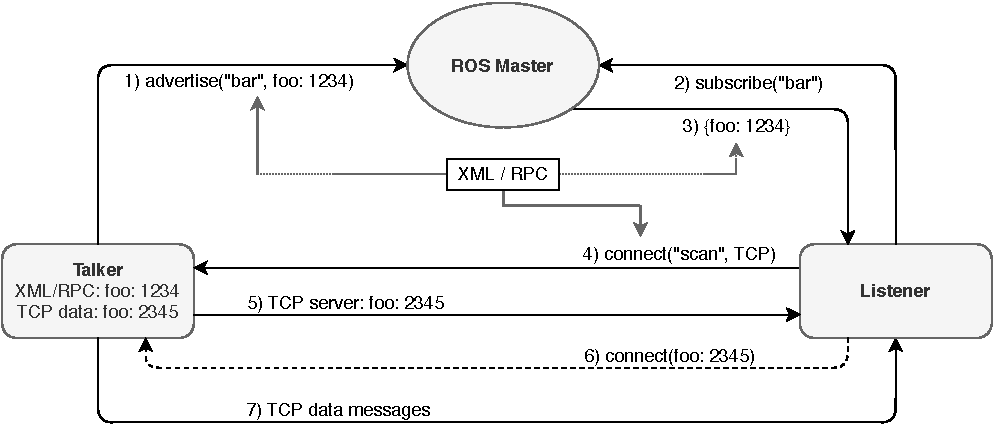
\includegraphics[width=0.9\textwidth]{images/ROSexample2.pdf}
	\caption{Example of nodes and topic communication}
	\label{fig:ros-nodes-topics}
\end{figure}

The reason to choose ROS for the development of robotics applications resides mainly in its high modularity. Furthermore it is a well known standard in the scientific community of the robotics researches and developers.




\subsection{NVIDIA Isaac SDK}
The Isaac SDK is the main software toolkit provided by NVIDIA and allows developers to brought new opportunities for developing robotics solutions as well as researching topics in this field. As described in \cite{ISAAC} it's comprised of the following:
\begin{itemize}
	\item Isaac Robot Engine: A framework which allows you to easily write modular applications and deploy them on your robots.
	\item Isaac GEMs: A collection of robotics algorithms from planning to perception, most of them GPU-accelerated.
	\item Applications: Various example applications from basic samples which show specific features to applications that facilitate complicated robotics use cases.
	\item Isaac Sim for Navigation: A powerful virtual robotics laboratory and a high-fidelity 3D world simulator that accelerates research, design, and development by reducing cost and risk.
\end{itemize}

The main reasons we would consider to use this platform reside in its high modularity and high performance solutions that it is able to offer on NVIDIA Jetson platforms.
Others important reasons to adopt this solution are related the \textbf{C API} that allows the communication with Isaac apps from languages other than C++, and the \textbf{ROS bridge} that offers the capability to interact with ROS nodes applications.

%TODO put an image that shows the Isaac architecture

\subsection{CoppeliaSim}
From the creators of V-Rep \cite{VREP}, CoppeliaSim \cite{coppeliaSim} seems to be the definitive solution for development of robotics applications.
The robot simulator CoppeliaSim, with integrated development environment, is based on a distributed control architecture: each object/model can be individually controlled via an embedded script, a plugin, ROS nodes, BlueZero nodes, remote API clients, or a custom solution. This makes CoppeliaSim very versatile and ideal for multi-robot applications. Controllers can be written in C/C++, Python, Java, Lua, Matlab, Octave or Urbi.
CoppeliaSim can be used as a stand-alone application or can easily be embedded into a main client application: its small footprint and elaborate API makes CoppeliaSim an ideal candidate to embed into higher-level applications. An integrated Lua script interpreter makes CoppeliaSim an extremely versatile application, leaving the freedom to the user to combine the low/high-level functionalities to obtain new high-level functionalities.




%%%%%%%%%%%%%%%%%%%%%%%%%%%%%%%%%%%%
\section{Docker} %TODO cite book
While container technologies have been around for a long time, they have become more widely known with the rise of the Docker container platform. Docker was the first container system that made containers easily portable across different machines. It simplifies the process of packaging up not only the application but also all its libraries and other dependencies, even the whole OS file system, into a simple, portable package that can be used to provision the application to any other machine running Docker. When you run an application packaged with Docker, it sees the exact filesystem contents that you have bundled with it. It sees the same files whether it is running on your development machine or a production machine, even if it the production server is running a completely different Linux OS. The application will not see anything from the server it is running on, so it does not matter if the server has a completely different set of installed libraries compared to your development machine.
This is similar to creating a VM image by installing an operating system into a VM, installing the app inside it, and then distributing the whole VM image around and running it. Docker achieves the same effect, but instead of using Virtual Machines (VMs) to achieve app isolation, it uses Linux container technologies to provide (almost) the same level of isolation that VMs do. Instead of using big monolithic VM images, it uses container images, which are usually smaller.

\subsection{Understanding Docker Concepts}
Docker is a platform for packaging, distributing, and running applications. It allows you to package your application together with its whole environment. This can be either a few libraries that the app requires or even all the files that are usually available on the filesystem of an installed operating system. Docker makes it possible to transfer this package to a central repository from which it can then be transferred to any computer running Docker and executed there.
Three main concepts in Docker comprise this scenario:

\begin{itemize}
	\item \textbf{Images}: A Docker-based container image is something you package your application and its environment into. It contains the filesystem that will be available to the application and other metadata, such as the path to the executable that should be executed when the image is run.
	\item \textbf{Registries}: A Docker Registry is a repository that stores your Docker images and facilitates easy sharing of those images between different people and computers. When you build your image, you can either run it on the computer you have built it on, or you can push (upload) the image to a registry and then pull (download) it on another computer and run it there. Certain registries are public, allowing anyone to pull images from it, while others are private, only accessible to certain people or machines.
	\item \textbf{Containers}: A Docker-based container is a regular Linux container created from a Docker-based container image. A running container is a process of the host on which Docker is running, but it is completely isolated from both the host and all other processes running on it. The process is also resource-constrained, meaning that it can only access and use the amount of resources (CPU, RAM, and so on) that are allocated to it.
\end{itemize}

Figure \ref{fig:dockerflow} shows all three concepts and how they relate to each other. The developer first builds an image and then pushes it to a registry. The image is thus available to anyone who can access the registry. They can then pull the image to any other machine running Docker and run the image. Docker creates an isolated container based on the image and runs the binary executable specified as part of the image.
Docker images are composed of layers. Different images can contain the exact same layers because every Docker image is built on top of another image and two different images can both use the same parent image as their base. This speeds up the distribution of images across the network, because layers that have already been transferred as part of the first image do not need to be transferred again when transferring the other image.
But layers do not only make distribution more efficient, they also help reduce the storage footprint of images. Each layer is only stored once. Two containers created from two images based on the same base layers can therefore read the same files, but if one of them writes over those files, the other one does not see those changes. Therefore, even if they share files, they are still isolated from each other. This works because container image layers are read-only. When a container is run, a new writeable layer is created on top of the layers in the image. When the process in the container writes to a file located in one of the underlying layers, a copy of the whole file is created in the top-most layer and the process writes to the copy.

\begin{figure}[tbp]
	\centering
	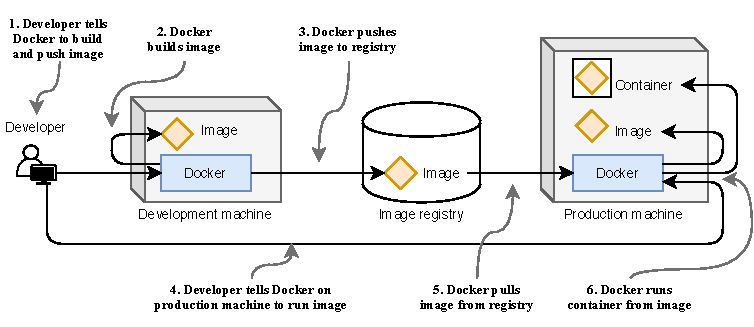
\includegraphics[width=0.9\textwidth]{images/dockerflow.pdf}
	\caption{Docker images, registries, and containers.}
	\label{fig:dockerflow}
\end{figure}

\subsection{Portability Limitations of Container Images}
In theory, a container image can be run on any Linux machine running Docker, but one small caveat exists, one related to the fact that all containers running on a host use the host's Linux kernel. If a containerized application requires a specific kernel version, it may not work on every machine. If a machine runs a different version of the Linux kernel or does not have the same kernel modules available, the app cannot run on it.

While containers are much more lightweight compared to VMs, they impose certain constraints on the apps running inside them. VMs have no such constraints, because each VM runs its own kernel.
And it is not only about the kernel. It should also be clear that a containerized app built for a specific hardware architecture can only run on other machines that have the same architecture. It is not possible containerize an application built for the x86 architecture and expect it to run on an ARM-based machine because it also runs Docker. You still need a Virtual Machine for that.
It is very important to understand that Docker itself does not provide process isolation. The actual isolation of containers is done at the Linux kernel level using kernel features such as Linux Namespaces and cgroups. Docker only makes it easy to use those features.

%TODO inderire la parte di rete di docker

%%%%%%%%%%%%%%%%%%%%%%%%%%%%%%%%%%%%
\section{Kubernetes} \label{sec:kubernetesbackground}
As the number of deployable application components in your system grows, it becomes harder to manage them all. Google was probably the first company that realized the need of a much better way to deploy and manage their software components and their infrastructure to scale globally. It is one of only a few companies in the world that runs hundreds of thousands of servers and has had to deal with managing deployments on such a massive scale. This has forced them to develop solutions for making the development and deployment of thousands of software components manageable and cost-efficient.


\subsection{What is Kubernetes}
Kubernetes is a software system that allows you to easily deploy and manage containerized applications on top of it. It relies on the features of Linux containers to run heterogeneous applications without having to know any internal details of these applications and without having to manually deploy these applications on each host. Because these apps run in containers, they do not affect other apps running on the same server, which is critical when you run applications for completely different organizations on the same hardware.
Kubernetes enables you to run your software applications on thousands of computer nodes as if all those nodes were a single, enormous computer.
Deploying applications through Kubernetes is always the same, whether your cluster contains only a couple of nodes or thousands of them. The size of the cluster makes no difference at all. Additional cluster nodes simply represent an additional amount of resources available to deployed apps.

\begin{figure}[tbp]
	\centering
	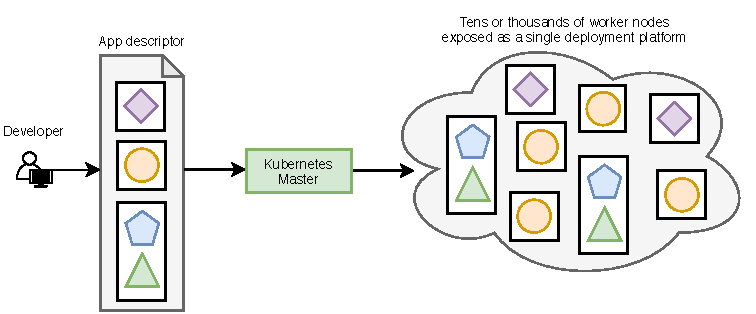
\includegraphics[width=0.9\textwidth]{images/kubernetesmain.pdf}
	\caption{Kubernetes exposes the whole datacenter as a single deployment platform.}
	\label{fig:kubernetesmain}
\end{figure}

Figure \ref{fig:kubernetesmain} shows the simplest possible view of a Kubernetes system. The system is composed of a master node and any number of worker nodes. When the developer submits a list of apps to the master, Kubernetes deploys them to the cluster of worker nodes. What node a component lands on does not (and should not) matter neither to the developer nor to the system administrator.

\subsection{Architecture of a Kubernetes cluster}
A Kubernetes cluster is composed of many nodes, which can be split into two types.
\begin{itemize}
	\item The \textit{master} node, which host the \textit{Kubernetes Control Plane} that controls and manages the whole Kubernetes system.
	\item Worker \textit{nodes} that run the actual applications you deploy.
\end{itemize}

The \textit{Control Plane} is what controls the cluster and makes it function.
It consists of multiple components that can run on a single master node or be split across multiple nodes and replicated to ensure high availability. These components are:
\begin{itemize}
	\item The Kubernetes \textit{API Server}, which you and the other Control Plane components communicate with.
	\item The \textit{Scheduler}, which schedules your apps (assigns a worker node to each deployable component of your application).
	\item The \textit{Controller Manager}, which performs cluster-level functions, such as replicating components, keeping track of worker nodes, handling node failures, and so on.
	\item \textit{etcd}, a reliable distributed data store that persistently stores the cluster configuration. 
\end{itemize}

The components of the Control Plane hold and control the state of the cluster, but they do not run your applications. This is done by the (worker) nodes.

The worker nodes are the machines that run your containerized applications. The task of running, monitoring, and providing services to your applications is done by the following components:
\begin{itemize}
	\item Docker, rkt, or another container runtime, which runs your containers.
	\item The Kubelet, which talks to the API server and manages containers on its node.
	\item The Kubernetes Service Proxy (kube-proxy), which load-balances network traffic
	between application components.
\end{itemize}
Figure \ref{fig:kubecluster} shows the components running on these two sets of nodes.


\begin{figure}[tbp]
	\centering
	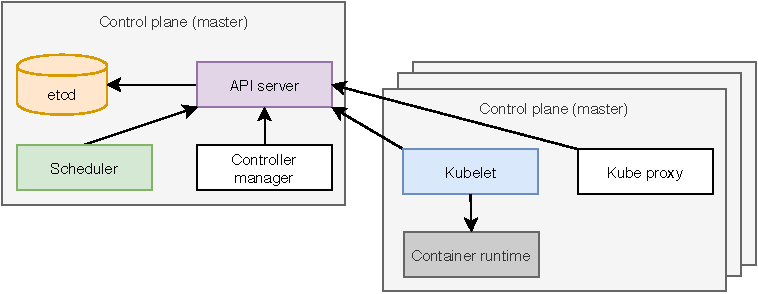
\includegraphics[width=0.9\textwidth]{images/kubecluster.pdf}
	\caption{The components that make up a Kubernetes cluster.}
	\label{fig:kubecluster}
\end{figure}



\subsection{Running an application in Kubernetes}
To run an application in Kubernetes, you first need to package it up into one or more container images, push those images to an image registry, and then post a description of your app to the Kubernetes API server.

The description includes information such as the container image or images that contain your application components, how those components are related to each other, and which ones need to be run co-located (together on the same node) and which do not. For each component, you can also specify how many copies (or replicas) you want to run. Additionally, the description also includes which of those components provide a service to either internal or external clients and should be exposed through a single IP address and made discoverable to the other components.
When the API server processes your app's description, the Scheduler schedules the specified groups of containers onto the available worker nodes based on computational resources required by each group and the unallocated resources on each node at that moment. The Kubelet on those nodes then instructs the Container Runtime (Docker, for example) to pull the required container images and run the containers.

\begin{figure}[tbp]
	\centering
	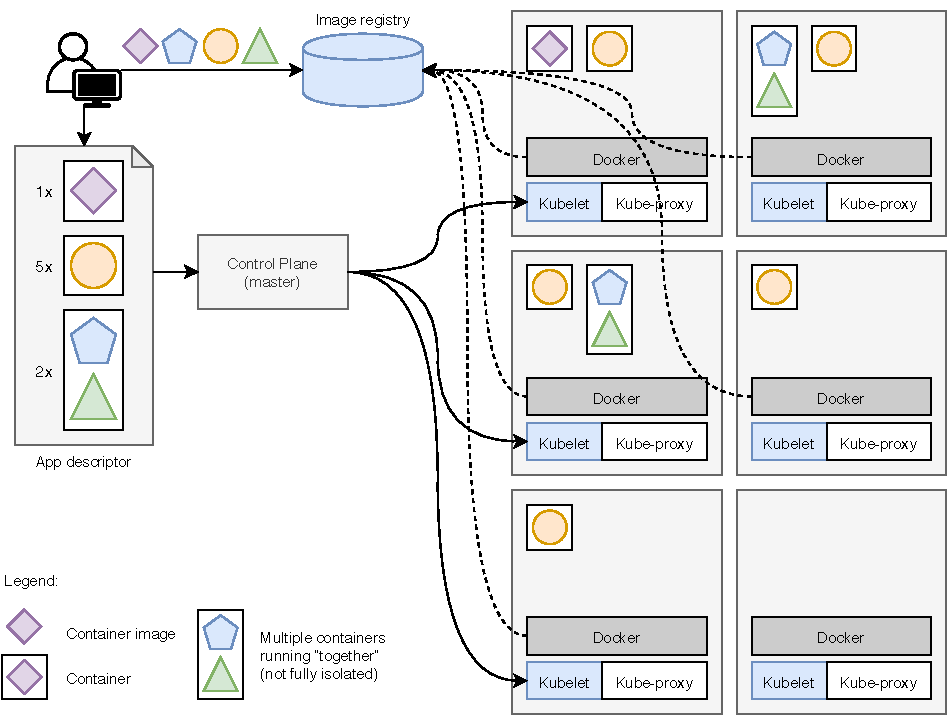
\includegraphics[width=0.9\textwidth]{images/kubedockeroverview.pdf}
	\caption{A basic overview of the Kubernetes architecture and an application running on top of it.}
	\label{fig:kubedockeroverview}
\end{figure}

Figure \ref{fig:kubedockeroverview} gives a better understanding of how applications are deployed in Kubernetes. The app descriptor lists four containers, grouped into three sets (these sets are called pods). The first two pods each contain only a single container, whereas the last one contains two containers. This means both containers need to run co-located and shouldn't be isolated from each other. Next to each pod, you also see a number representing the number of replicas of each pod that need to run in parallel. After submitting the descriptor to Kubernetes, it will schedule the specified number of replicas of each pod to the available worker nodes. The Kubelets on the nodes will then tell Docker to pull the container images from the image registry and run the containers.


\subsection{Monitoring of Performance}
Properly setting resource requests and limits within a Pod, is crucial for getting the most out of your Kubernetes cluster. If requests are set too high, your cluster nodes will be underutilized and you will be throwing money away. If you set them too low, your apps will be CPU-starved or even killed by the Out Of Memory (OOM) Killer. How do you find the sweet spot for requests and limits?
You find it by monitoring the actual resource usage of your containers under the expected load levels. Once the application is exposed to the public, you should keep monitoring it and adjust the resource requests and limits if required.
Since Kubernetes v1.18 monitoring is split into two pipelines:
\begin{itemize}
	\item A \textbf{core metrics pipeline} consisting of Kubelet, a resource estimator, a slimmed-down Heapster called metrics-server, and the API server serving the master metrics API. These metrics are used by core system components, such as scheduling logic (e.g. scheduler and horizontal pod autoscaling based on system metrics) and simple out-of-the-box UI components (e.g. kubectl top). 
	\item A \textbf{monitoring pipeline} used for collecting various metrics from the system and exposing them to end-users, as well as to the Horizontal Pod Autoscaler (for custom metrics) and Infrastore via adapters. Users can choose from many monitoring system vendors, or run none at all. In open-source, Kubernetes will not ship with a monitoring pipeline, but third-party options will be easy to install. Pipelines will typically consist of a per-node agent and a cluster-level aggregator. 
\end{itemize}
The architecture of the core metrics pipeline is illustrated in figure \ref{fig:metricspipe}.
\begin{figure}[tbp]
	\centering
	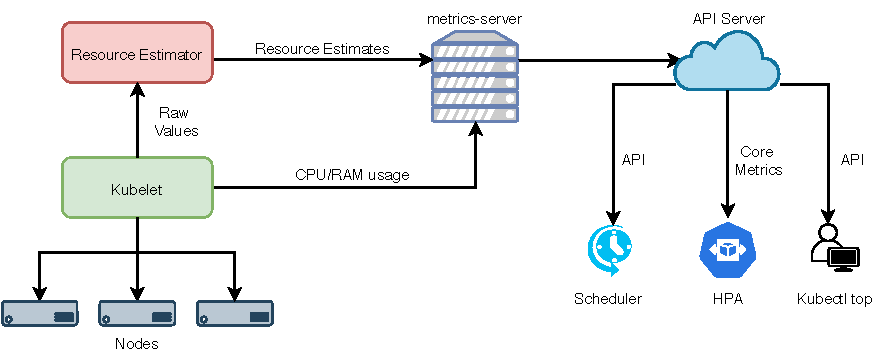
\includegraphics[width=0.9\textwidth]{images/k8smonitor.pdf}
	\caption{Core Metrics pipeline.}
	\label{fig:metricspipe}
\end{figure}
The interaction with these API can be performed through the command line tool or into graphical web user interfaces web dashboard provided by Google.
The dashboard allows you to list all the Pods, Replication Controllers, Services, and other objects deployed in your cluster, as well as to create, modify, and delete them. Figure \ref{fig:ui-dashboard} shows the dashboard that we are talking about.

\begin{figure}[bp]
	\centering
	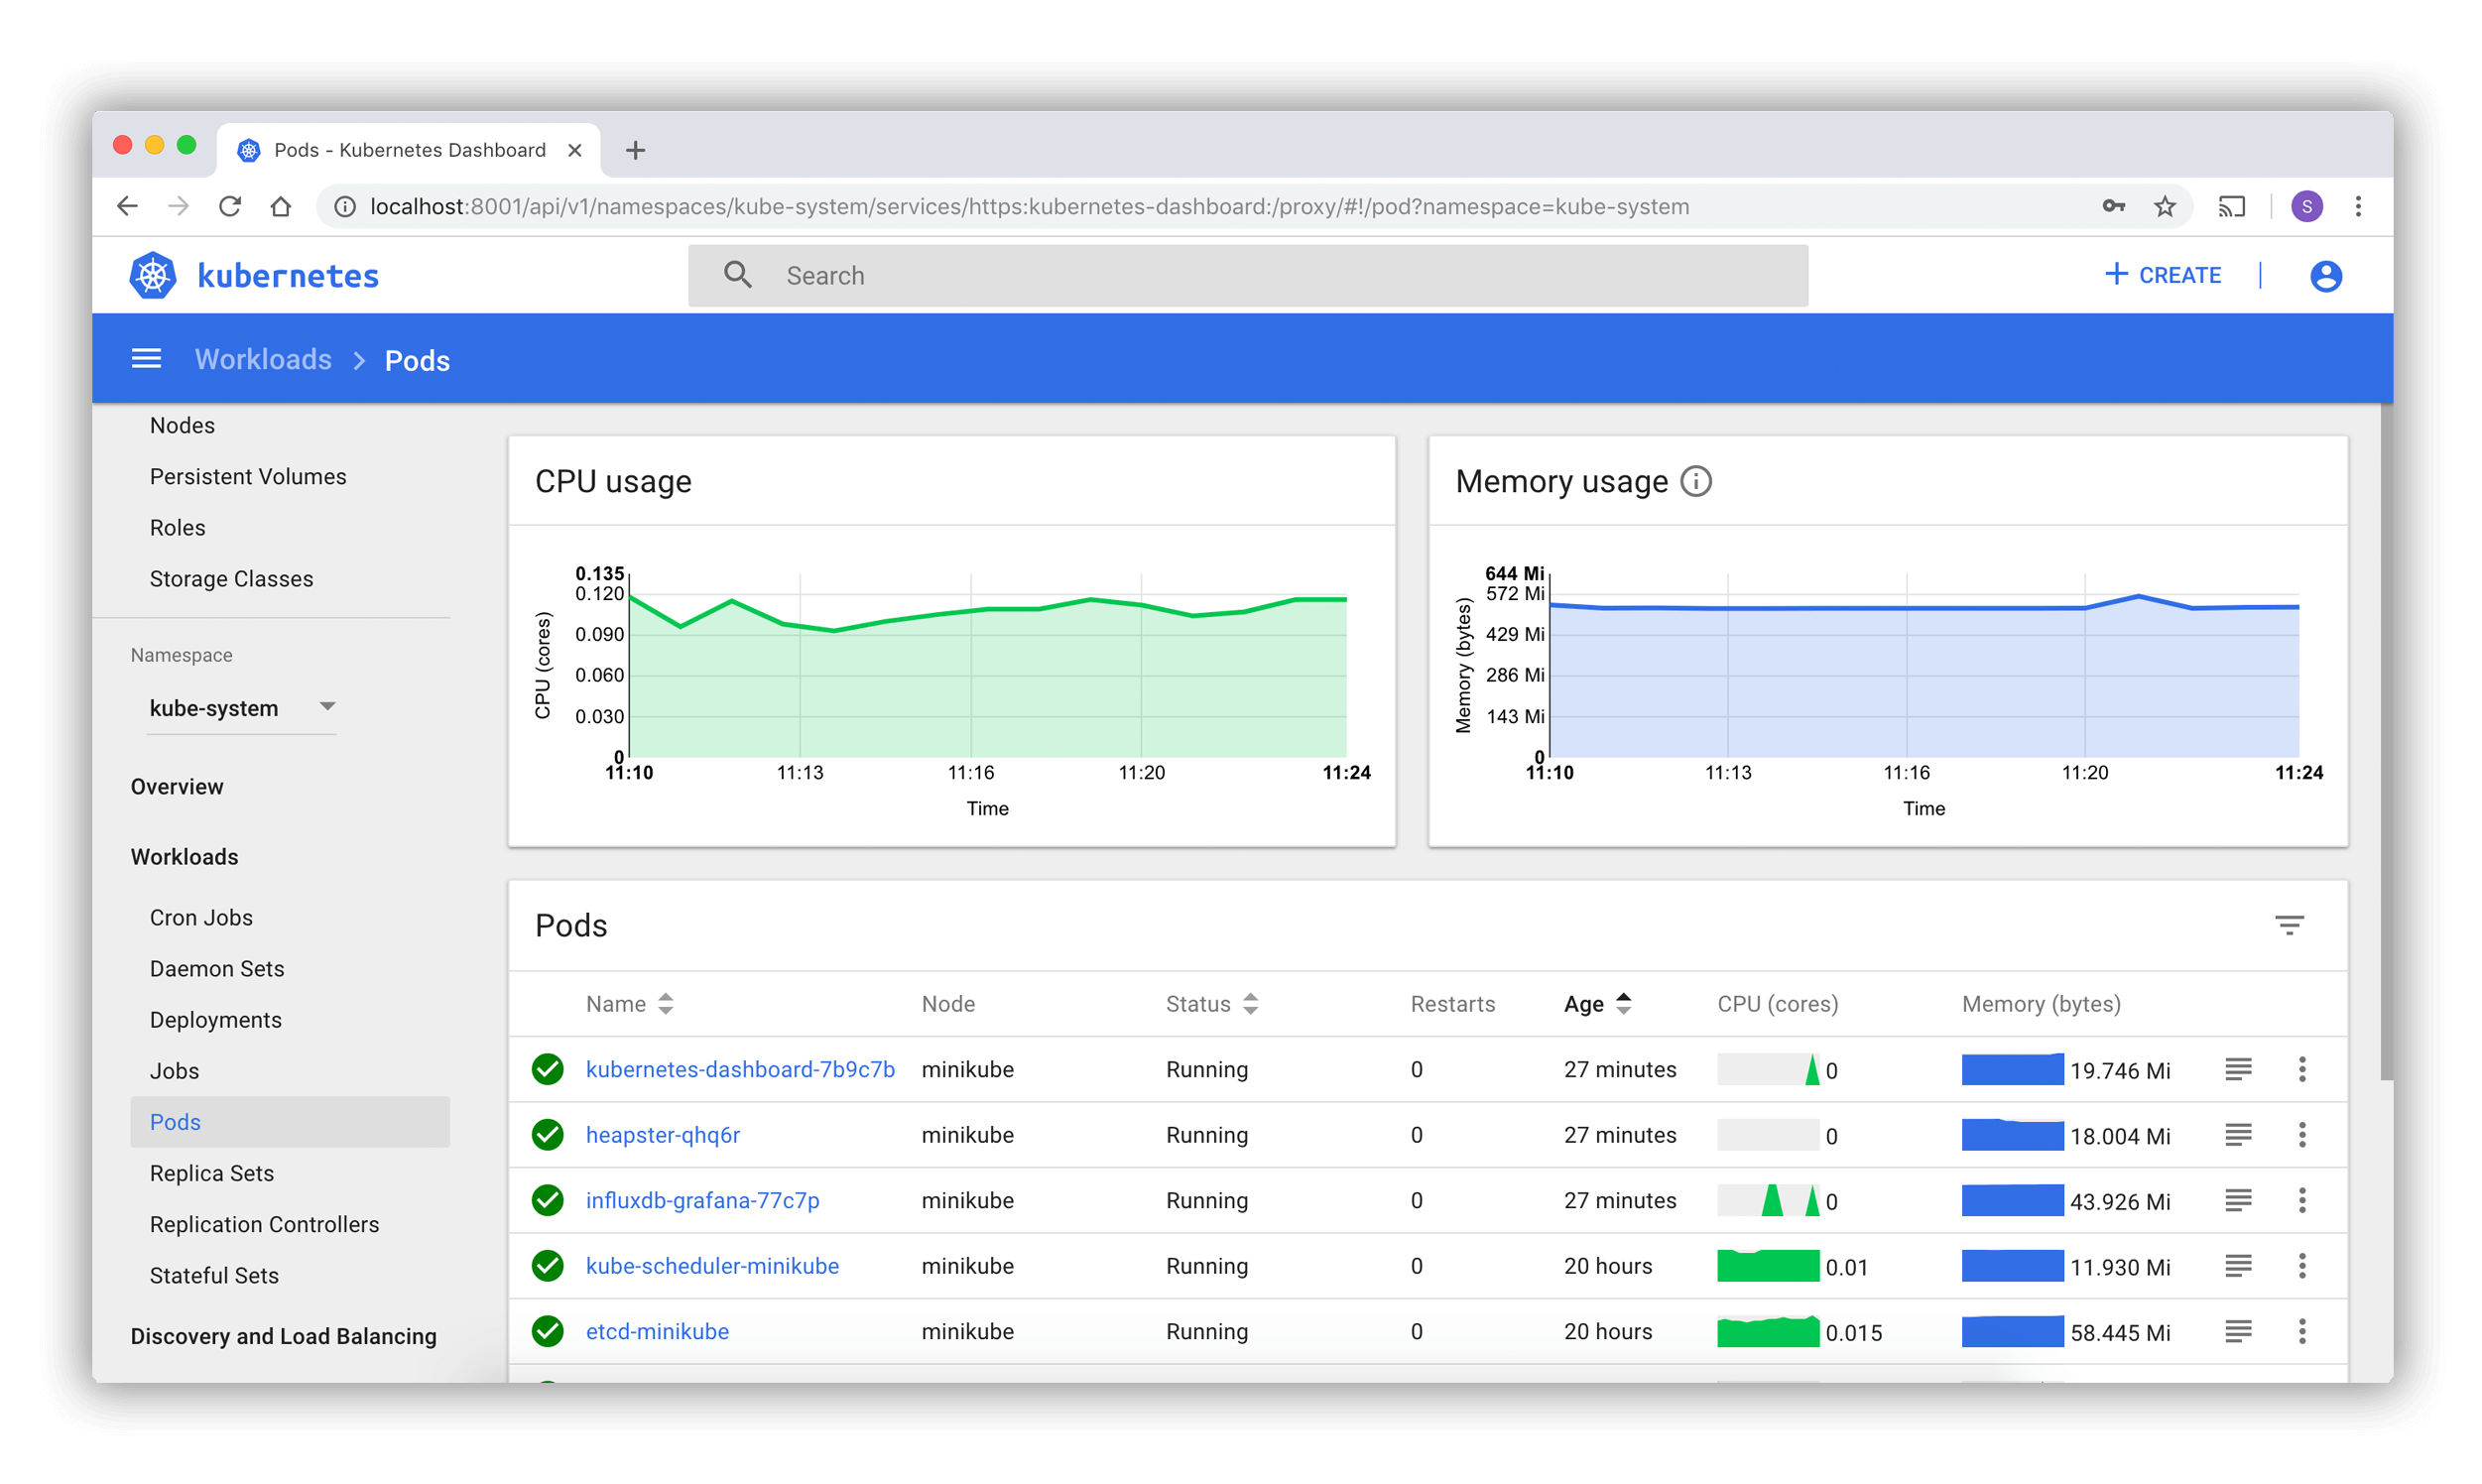
\includegraphics[width=\textwidth]{images/ui-dashboard.png}
	\caption{Kubernetes Dashboard.}
	\label{fig:ui-dashboard}
\end{figure}



%%%%%%%%%%%%%%%%%%%%%%%%%%%%%%%%%%%%
\section{KubeEdge} \label{sec:kubeedgebackground}
KubeEdge is an open source system extending native containerized application orchestration and device management to hosts at the Edge. It is built upon Kubernetes and provides core infrastructure support for networking, application deployment and metadata synchronization between cloud and edge. It also supports MQTT and allows developers to author custom logic and enable resource constrained device communication at the Edge.

\subsection{Motivation}
With KubeEdge it is easy to get and deploy existing complicated machine learning, image recognition, event processing and other high level applications to the Edge. With business logic running at the Edge, much larger volumes of data can be secured and processed locally where the data is produced. With data processed at the Edge, the responsiveness is increased dramatically and data privacy is protected.
The advantages of KubeEdge include mainly:
\begin{itemize}
	\item \textbf{Edge Computing}: with business logic running at the Edge, much larger volumes of data can be secured and processed locally where the data is produced. This reduces the network bandwidth requirements and consumption between Edge and Cloud. This increases responsiveness, decreases costs, and protects customer's data privacy.
	\item \textbf{Simplified development}: Developers can write regular http or mqtt based applications, containerize these, and run them anywhere - either at the Edge or in the Cloud - whichever is more appropriate.
	\item \textbf{Kubernetes-native support}: With KubeEdge, users can orchestrate apps, manage devices and monitor app and device status on Edge nodes just like a traditional Kubernetes cluster in the Cloud.
	\item \textbf{Abundant applications}: It is easy to get and deploy existing complicated machine learning, image recognition, event processing and other high level applications to the Edge.
\end{itemize}

In the era of Internet of Thing (IoT), billions of sensors and actuators are deployed worldwide. To manage the IoT devices and process data with cloud computing resource,
Cloud providers such as Amazon AWS and Microsoft Azure are developing the IoT platform and are providing services or solutions on their respective cloud environments.

Most IoT platforms employ a Publisher/Subscriber (Pub/Sub) brokers such as MQTT \cite{mqttpubsub} or AMQP to provide the communication channel between IoT devices and Cloud services, like Azure IoT Hub. Pub/Sub protocol such as MQTT is suitable for asynchronous communication between edge devices and cloud services. However it does not support synchronous RPC based communication, for the increased need as more and more computation tasks \cite{bigdataedge}\cite{edgerealtime} move to the edges and tightly integrate with services in the cloud.
One common scenario for RPC based communication is the cloud native micro-service based application. With micro-service architecture, an application is designed into multiple micro services, each of which is deployed and managed independently. These micro services communicate each other usually through REST/HTTP protocol. When some of the micro services run on the edge nodes and need to communicate with those in the cloud, it requires the one network address space for both edge nodes and server instances in the cloud.
This is where current edge computing solutions break down, partly due to the asynchronous Pub/Sub based MQTT protocol \cite{kubeedgeinspection}.
KubeEdge leverages Kubernetes container platform to provide RPC based communication channel between edge and cloud, the runtime execution environment of containers and Serverless functions, as well as a mechanism to sync and store metadata to support self-management of an application running on the edge in an offline scenario.  

Furthermore, since KubeEdge is built upon Kubernetes all the tools available in Kubernetes are also available in KubeEdge. Therefore we can benefit of all the monitoring platforms such as the dashboard and metric-server shown in the previous section.

\subsection{Kubeedge Architecture}
As shown in Figure \ref{fig:kubeedge-arch}, KubeEdge is a multi-tenant infrastructure platform for edge computing.
The platform includes the following components, excluding Kubernetes.
\begin{itemize}
	\item \textbf{Edged}: an agent that runs on edge nodes and manages containerized applications.
	\item \textbf{EdgeHub}: a web socket client responsible for interacting with Cloud Service for edge computing (like Edge
	Controller as in the KubeEdge Architecture). This includes syncing cloud-side resource updates to the edge and
	reporting edge-side host and device status changes to the cloud.
	\item \textbf{CloudHub}: A web socket server responsible for watching changes at the cloud side, caching and sending
	messages to EdgeHub.
	\item \textbf{EdgeController}: an extended kubernetes controller which manages edge nodes and pods metadata so that the
	data can be targeted to a specific edge node.
	\item \textbf{EventBus}: an MQTT client to interact with MQTT servers (mosquitto), offering publish and subscribe capabilities to other components.
	\item \textbf{DeviceTwin}: responsible for storing device status and syncing device status to the cloud. It also provides query
	interfaces for applications.
	\item \textbf{MetaManager}: the message processor between edged and edgehub. It is also responsible for storing/retrieving
	metadata to/from a lightweight database (SQLite).
\end{itemize}

\begin{figure}[tbp]
	\centering
	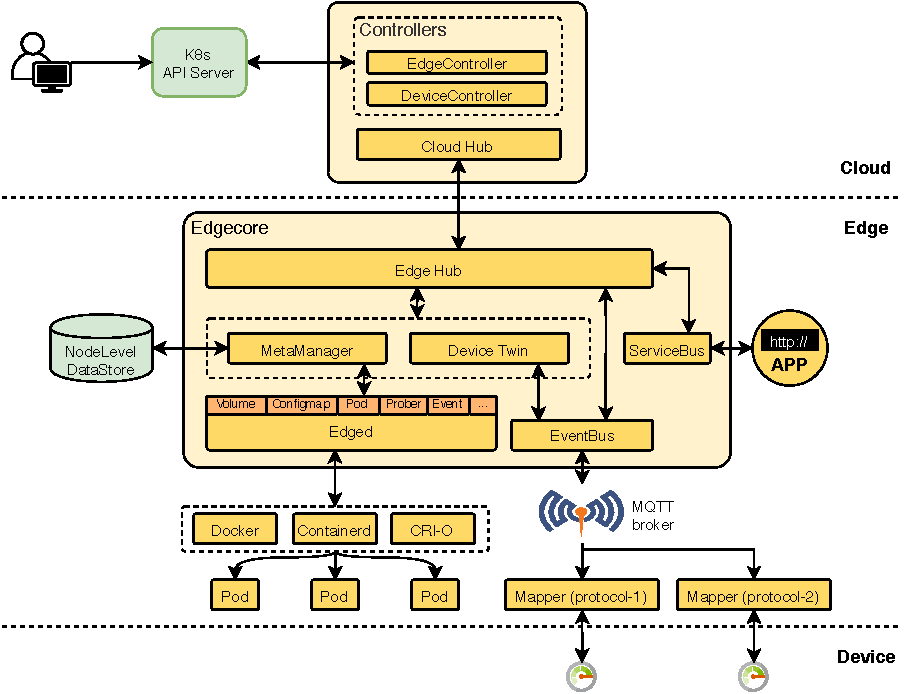
\includegraphics[width=\textwidth]{images/kubeedge-arch}
	\caption{KubeEdge Architecture.}
	\label{fig:kubeedge-arch}
\end{figure}




\clearpage
\thispagestyle{empty}